\newpage
\section*{Примеры работы программы:}
\begin{figure}[h]
    \centering
    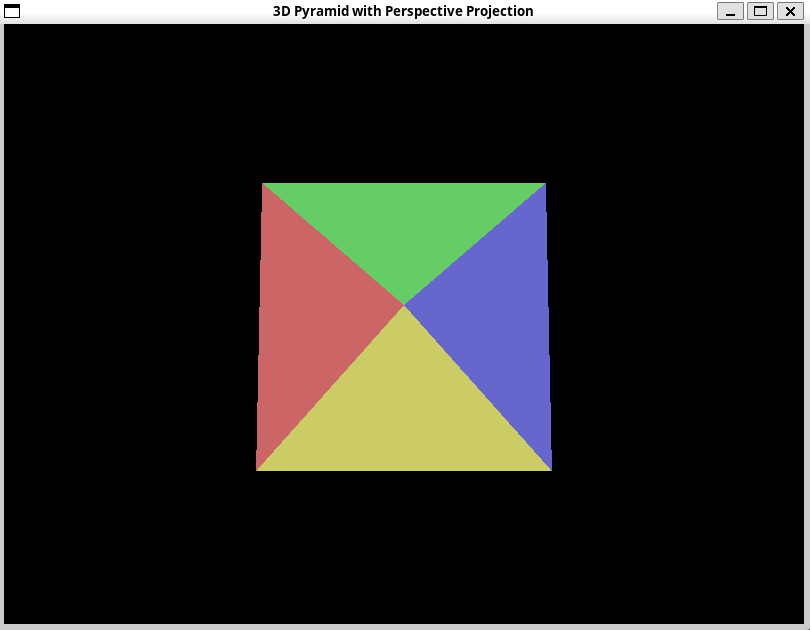
\includegraphics[width=0.8\textwidth]{lab2.1.png} % Путь к файлу фотографии
    \caption{Трёхмерная пирамида}
    \label{fig:lab2}
\end{figure}

\begin{figure}[h]
    \centering
    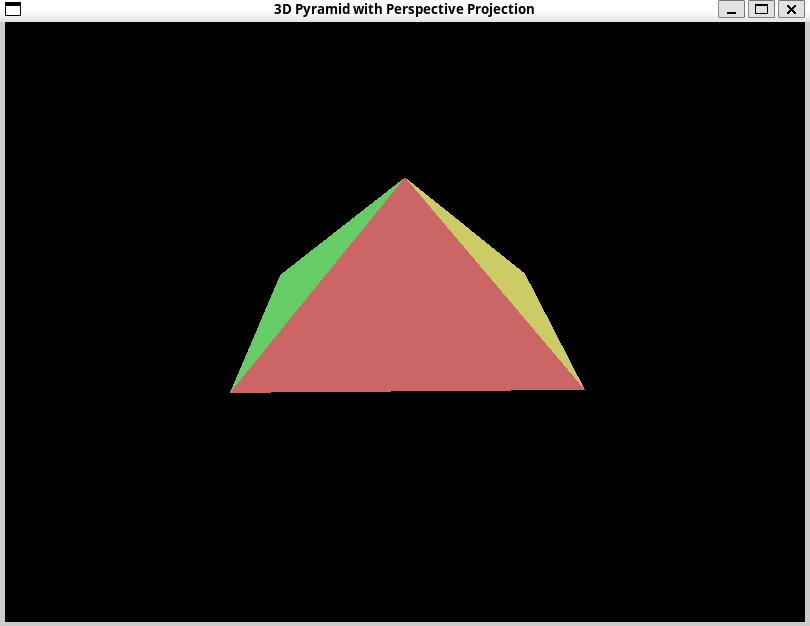
\includegraphics[width=0.8\textwidth]{lab2.2.png} % Путь к файлу фотографии
    \caption{Трансформация пирамиды}
    \label{fig:lab2}
\end{figure}

\clearpage

\section*{Результаты работы программы}

В результате выполнения программы был создан графический интерфейс для отображения трёхмерной пирамиды с использованием перспективной проекции. Программа предоставляет возможность управления положением, вращением и масштабированием пирамиды с помощью клавиш управления, а также отображает изменения в реальном времени.

\subsection*{Основные функции программы}
Программа реализует следующие возможности:
\begin{itemize}
    \item \textbf{Перемещение пирамиды:}
    \begin{itemize}
        \item \textbf{W} — перемещение вперёд.
        \item \textbf{S} — перемещение назад.
        \item \textbf{A} — перемещение влево.
        \item \textbf{D} — перемещение вправо.
    \end{itemize}
    \item \textbf{Вращение пирамиды:}
    \begin{itemize}
        \item \textbf{Q} — вращение против часовой стрелки по оси Y.
        \item \textbf{E} — вращение по часовой стрелке по оси Y.
        \item \textbf{I} — вращение вверх по оси X.
        \item \textbf{K} — вращение вниз по оси X.
    \end{itemize}
    \item \textbf{Масштабирование пирамиды:}
    \begin{itemize}
        \item \textbf{Z} — уменьшение масштаба.
        \item \textbf{X} — увеличение масштаба.
    \end{itemize}
    \item \textbf{Цветовая индикация:} Цвет пирамиды меняется в зависимости от направления трансформации:
    \begin{itemize}
        \item Перемещение — динамическое изменение цвета.
        \item Вращение — градиентные изменения цвета для визуализации движения.
    \end{itemize}
\end{itemize}

\subsection*{Графический интерфейс}
\begin{itemize}
    \item Пирамида отображается в окне размером $800 \times 600$ пикселей.
    \item В правом верхнем углу окна отображается информация о текущем состоянии пирамиды:
    \begin{itemize}
        \item Позиция центра пирамиды $(x, y, z)$.
        \item Угол вращения по каждой оси.
        \item Текущий масштаб.
    \end{itemize}
    \item Для отображения сцены используется OpenGL с настройкой перспективной проекции.
\end{itemize}

\subsection*{Пример работы программы}
\begin{enumerate}
    \item Изначальное состояние пирамиды: центр $(0, 0, -5)$, масштаб: $1.0$, углы поворота $(0^\circ, 0^\circ, 0^\circ)$.
    \item При нажатии клавиши \textbf{W}:
    \begin{itemize}
        \item Позиция изменилась на $(0, 0, -4.9)$.
        \item Цвет пирамиды изменился на градиентный оттенок (например, голубой).
    \end{itemize}
    \item При нажатии клавиш \textbf{A} и \textbf{Q}:
    \begin{itemize}
        \item Позиция изменилась на $(-0.1, 0, -4.9)$.
        \item Угол поворота вокруг оси Y стал $-5^\circ$.
        \item Цвет изменился на жёлтый градиент.
    \end{itemize}
    \item При нажатии клавиши \textbf{X}:
    \begin{itemize}
        \item Масштаб увеличился до $1.1$.
        \item Цвет остался неизменным.
    \end{itemize}
\end{enumerate}

\subsection*{Тестирование работы программы}
\begin{itemize}
    \item \textbf{Тестирование трансформаций:} Все действия успешно протестированы, и отображение в реальном времени выполнено корректно.
    \item \textbf{Производительность:} Частота обновления поддерживается на уровне $60$ кадров в секунду.
    \item \textbf{Устойчивость:} Ошибок и исключений во время выполнения программы не выявлено.
\end{itemize}

\subsection*{Выводы}
Программа успешно реализовала принципы трёхмерной графики с использованием OpenGL и SFML. Трансформации пирамиды работают стабильно, а графический интерфейс предоставляет пользователю полный контроль над объектом.
